\section{Sequence Diagram for movement}

On figure \ref{SquenceDiagramMovement} is shown the sequence of what happens when a person moves the player(avatar) on the screen. Before the player can be moved it is checked if the player got any actions left. The GameView will call the FirebaseHelper where it sets the newly updated PlayerList. This will then get updated asynchronously towards the database. 
Every player have then earlier made an eventListener that listens for changes, so when the database is changed all boards update automatically, by invoking setPlayerList on GameView.

\begin{figure}
	\centering
	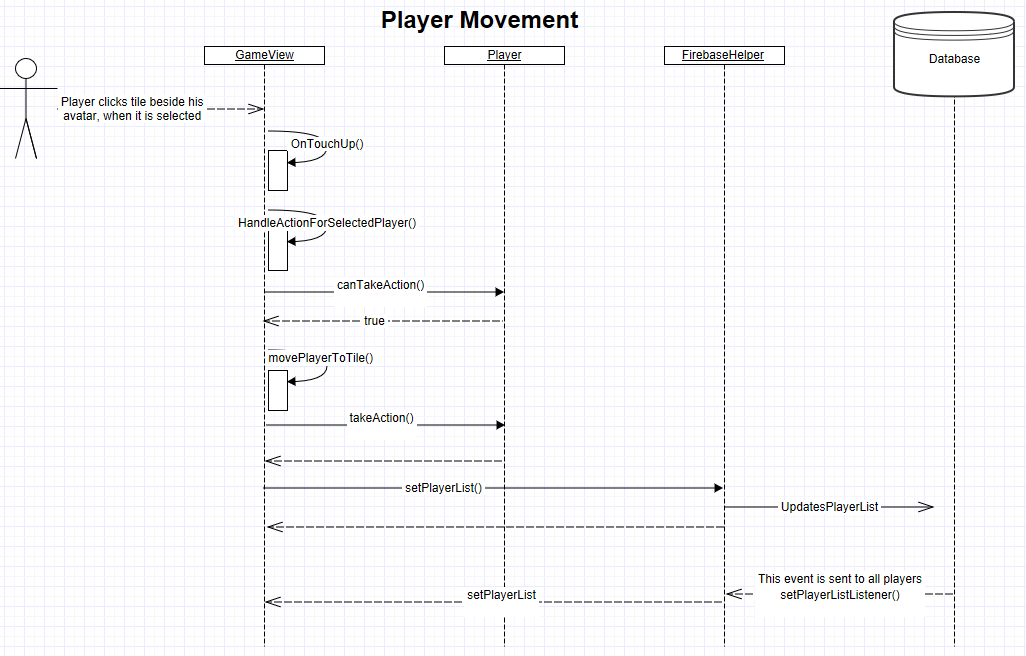
\includegraphics[width=0.8\textwidth]{images/SquenceDiagramMovement.PNG}
	\caption{Sequence Diagram for movement of player \label{SquenceDiagramMovement}}
\end{figure}